%The executive summary is a special chapter before the TOC
% See the other sections (e.g. Context) for more normal chapter headings
%%%%%%%%%%%%%%%%%%%%%%%%%%%%%%%%%%%%
% Call it Front Matter in TOC, as it will include Glossary and auto-generated TOC, LOF.
\chapter[Prelude]{Prelude}
\label{cha:front}
%\addcontentsline{toc}{section}{Executive Summary}
%%%%%%%%%%%%%%%%%%%%%%%%%%%%%%%%%%%%
%Begin the actual executive summary text. If you create any subsections you
%probably want to use  \section*{Section name}  with an asterisk, so they are not numbered.
% Note: to get proper looking quotes use two left/right single quotes: ``. . . ''

 \section{Executive Summary} 

In a world that is dynamic in almost every aspect, mobility is a necessity.  However, for persons that suffer from disabilities, their mobility can be severely limited.  Traveling with limited mobility can be a very difficult and burdening task, especially if it involves being within the small confines of an airplane.  Passengers that are faced with limited mobility or a disability have a different and often times worse experience than the average passenger throughout the entire flight experience.  How can we give all passengers the same experience? Creating a new travel system are essential for giving the same experience to all passengers and to give passengers with limited mobilitythe independence and control they lack today.

Embraer, the Brazilian airline manufacturer, decided to partner with Stanford University and the University of Sao Paulo to solve the problem of improving the entire air travel experience for persons with limited mobility. In collaboration, we started this journey toward a solution through extensive needfinding and benchmarking. The needfinding centered on conducting user interviews for both the disabled passenger and the flight crew, while benchmarking focused on analyzing analogous situations, patents, regulations, and current concepts and solutions in place today.

The research that was conducted during needfinding and benchmarking was instrumental in the approach we are taking toward a solution. The user interviews led us to the four themes we need to address with our solution. These themes are improving customer service, giving the user control and independence, and creating a non-discriminatory solution. The interviews with potential users revealed horror stories that dealt with customer service or the lack thereof. The solution space needs to create an environment that limits or improves the quality of the interactions between the flight crew and the passenger to prevent these horror stories from becoming a reality for future travelers. Independence and control were also instrumental in our findings. The users of our solution want to feel independent and in control of their situation even when they might need assistance. This leads our solution path to one that provides piece of mind to our user. Because wheelchairs often gets damaged when they are handled from the jet way to the cargo hold, wheelchair users are very anxious and spend their flight wondering if  their mobility device will make it safely to their destination. Finally, we realized that since passengers with disabilities have a condition that singles them out, we should focus on creating a product that is well designed with the user in mind and that lacks the dehumaninzing aspects that we see in cabin mobility aids today.

These themes were our driving forces for the critical function and critical experience prototypes we created to further explore our problem space. The team created a number of prototypes but really focused on the ones that solved this problem; one being a more incremental fix while the other addressed a more futuristic solutions. 

Our vision is to provide the wheelchair user with two products that address the main themes and the biggest painpoints. As mobility inside the cabin is an extremely uncomfortable and unsafe experience today, we want to give passengers a completely redesigned aisle chair that allows for improved customer service as well as increased passenger comfort and support. No longer do passengers need to be carried by airport personnel and risk injury since this redesigned aisle chair will allow the user to move inside the cabin and transfer independently from one seat to the next using either the lateral or frontal transfer options.  Having access to a more humane and versatile aisle chair will certainly revolutionize the flying experience for wheelchair users.

Beyond solving mobility inside the cabin, airport logistics concerning wheelchair storage must also be improved. It doesn't matter how delightful the flight experience was if a disabled passenger can't move once they arrive at their destination because their wheelchair is broken. We found that most of the damage to wheelchairs is incurred during the handling process so we have created a platform that allows handlers to manipulate any type of wheelchair, whether it's powered or manual, without having to touch the wheelchair itself. We are also using smart features that know who is responsible for the wheelchair and can detect any signs of mishandling. With this, we aim to reduce the number of damaged wheelchairs and improve the handing experience for airport personnel. 

We know that in order to provide wheelchair users with an enjoyable flying experience from beginning to end, our solution must provide them with absolute piece of mind concerning what happens to their mobility device when it is taken away from them and  a pleasant cabin experience that makes them feel independent, in control and not singled out. Both improvements, shown in Figure ref{fig:exec}  are necessary to truly redesigning the flying experience for people with reduced mobility. 

\begin{figure}[h]
\centering
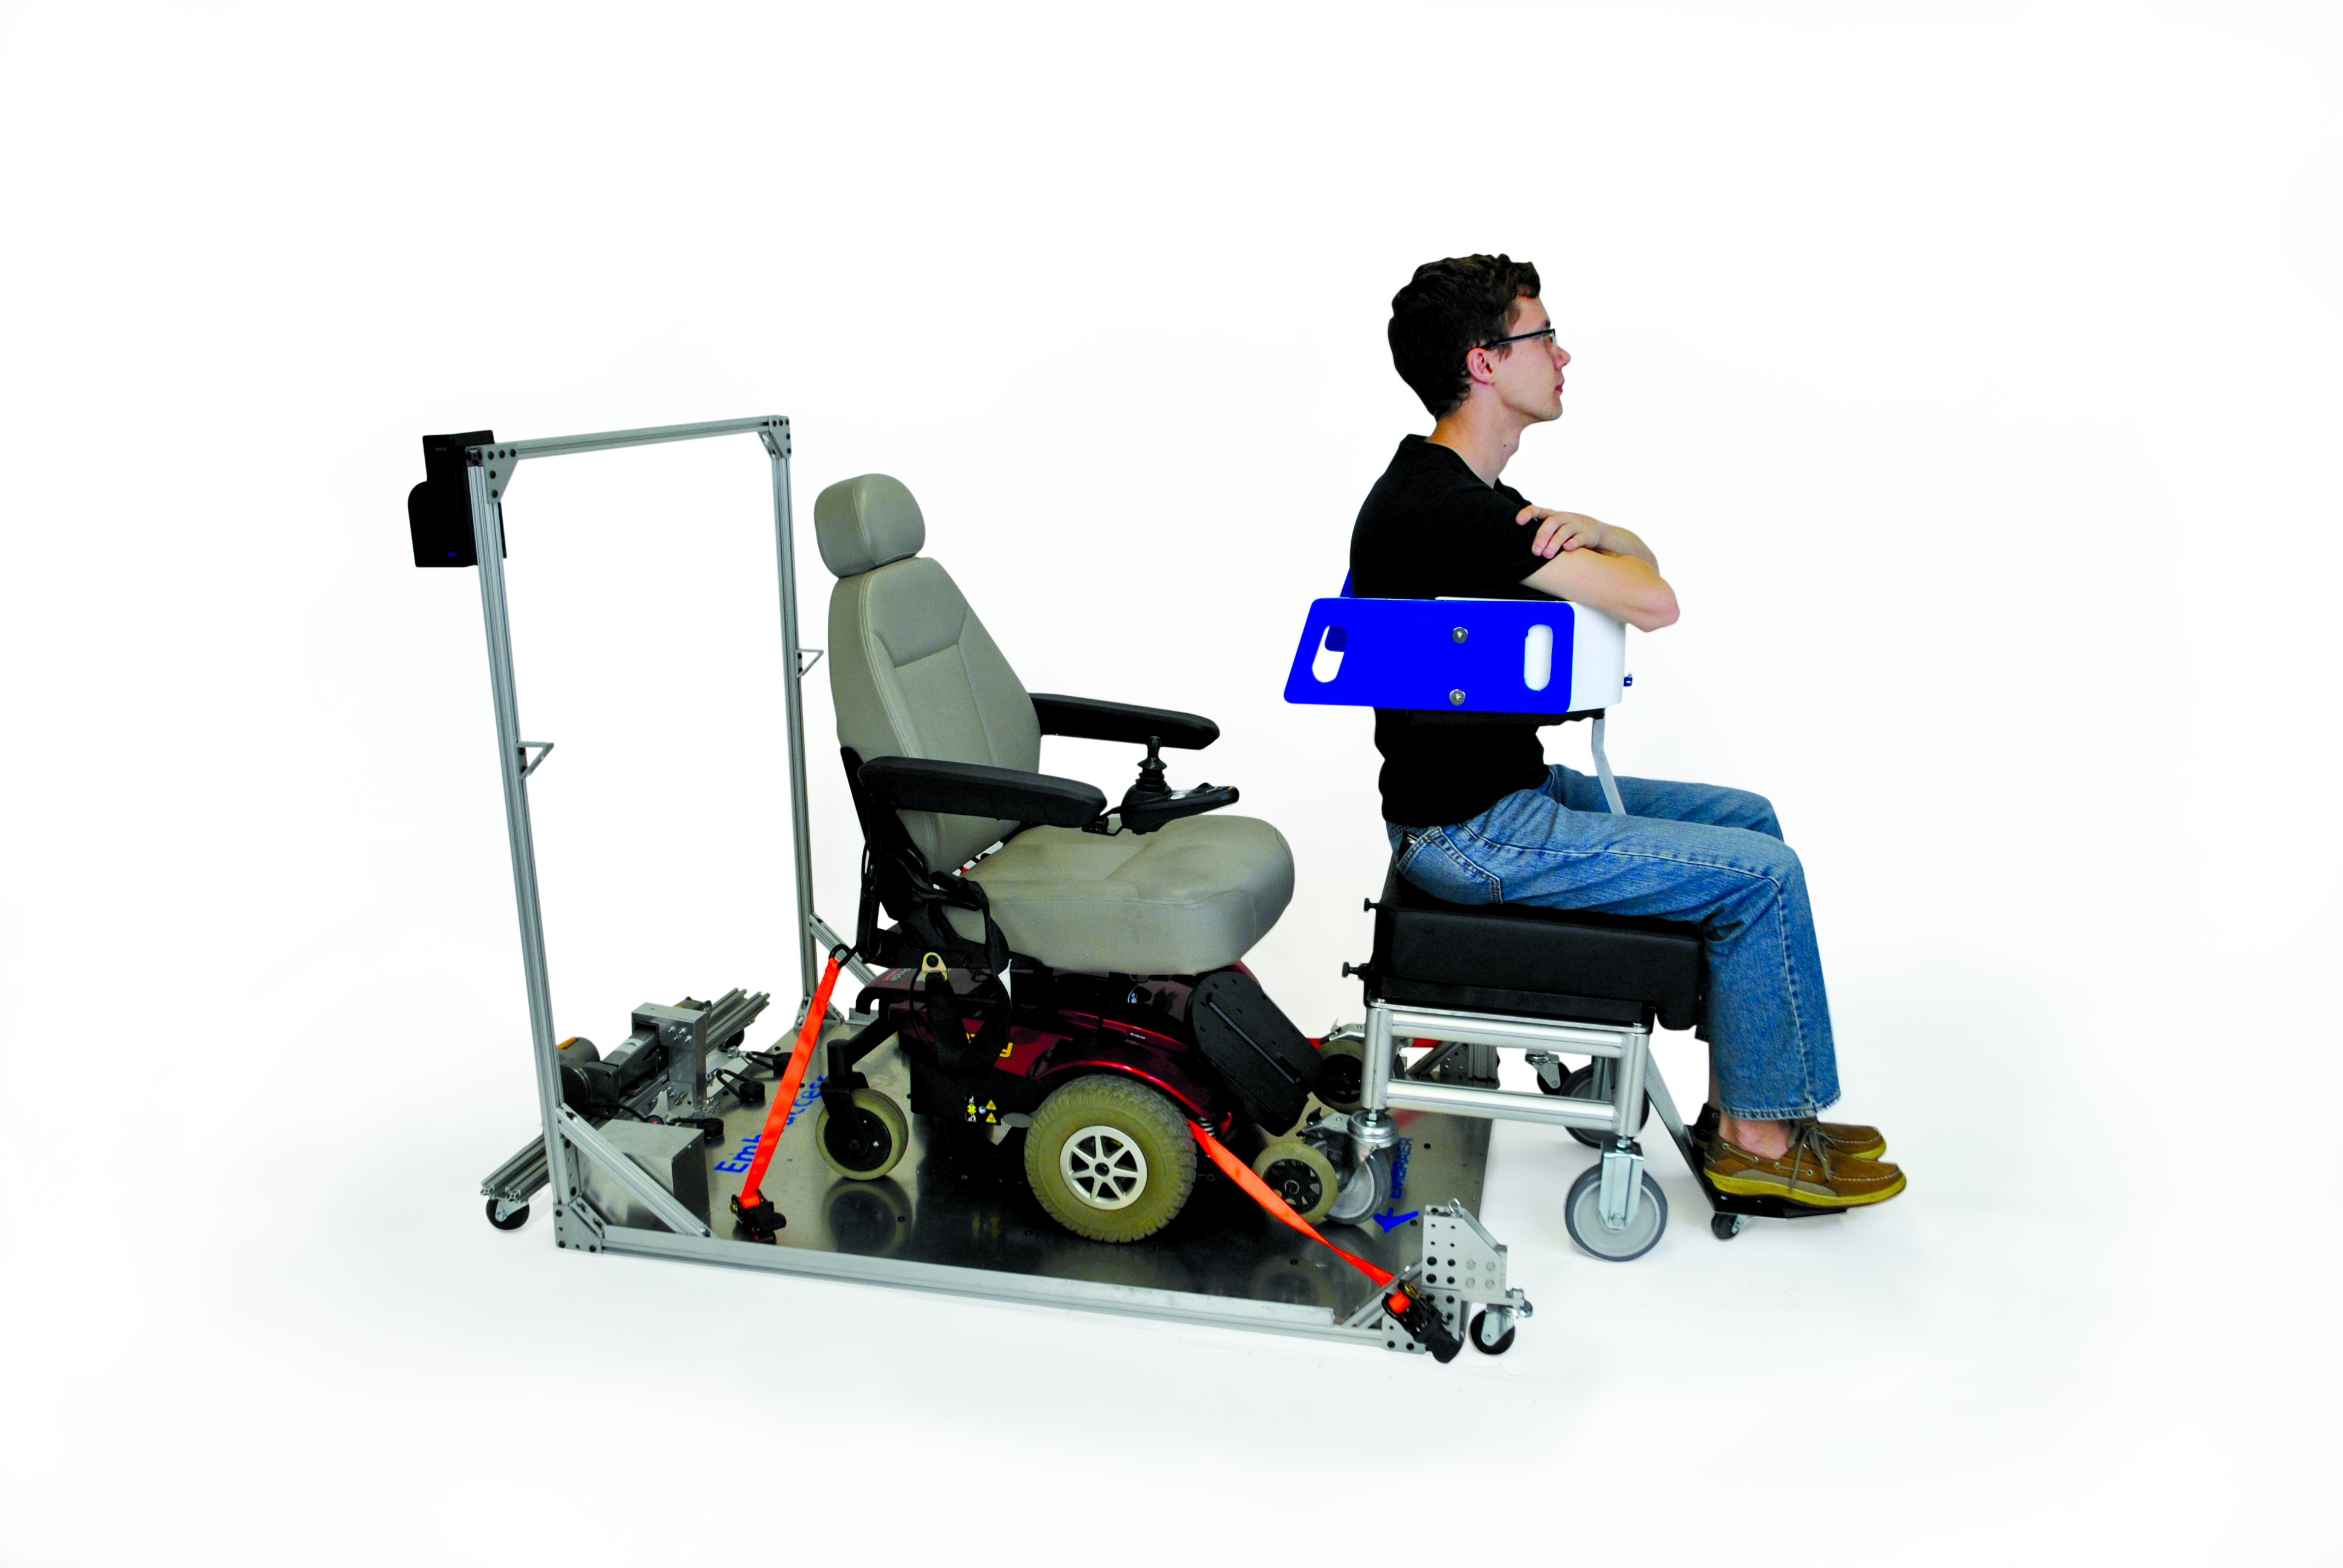
\includegraphics[width=13cm]{images/execsummary.jpg}
\caption{Both products enable a whole new experience for our users.}
\label{fig:exec}
\end{figure}


% add a picture of the whole system

%\section*{Glossary}

%\begin{list}{-}{}

%\end{list}

% Set up the Glossary. The template is looking for a file called
% "glossaryterms.tex" with glossary terms and definitions.
% You can either edit this file manually or you
% can use the Memoir glossary feature in which you insert items like
%   \glossary{glossary term}{our definition of what the term means}
% wherever you like, as you write your documentation.
% When you run the report through Latex, it will create a ".glo" file like
% "OurFallDocument.glo" which you can edit to create the file "glossaryterms.tex"
% There is also perl script I made which will do the formatting for you. 
%  perl Glo2Tex OurFallDocument.glo > glossaryterms.tex

\newpage
\section{Glossary}
%\addcontentsline{toc}{section}{Glossary}
\label{sec-glossary}
\begin{description}
  \item  \textbf{ADA:} Americans with Disabilities Act; one of America's most comprehensive pieces of civil rights legislation that prohibits discrimination against and guarantees people with disabilities have the same opportunities as everyone else to participate in the mainstream of American life.
  \item \textbf{ANAC:} Agencia Nacional de Aviação Civil – Brazilian National Agency of Civil Aviation
  \item  \textbf{Assistive Technology:} Assistive, adaptive, and rehabilitative devices for people with disabilities; promotes greater independence by enabling people to perform tasks that they were formerly unable to accomplish, or had great difficulty accomplishing.
  \item  \textbf{Benchmarking:} A standard by which something can be measured or judged.
  \item \textbf{Control:} The power to influence or direct either people's behavior or the course of events.
  \item \textbf{Dark Horse Prototype:} A device created during the winter quarter of ME310 that was ruled out in the fall quarter or undiscovered due to being “too risky” or “to difficult to complete”; emphasizes creative out-of-the-box thinking and exploring all of the design space for the project. 
  \item \textbf{Disability:} A physical or mental condition that limits a person's movements, senses, or activities.
  \item \textbf{EXPE:} The Stanford design fair that is held every year at the beginning of June. During this fair, all ME 310 teams present the work they have done throughout the year and show their final prototype.
  \item \textbf{FAA:} Federal Aviation Administration; United States national aviation authority whose mission is to provide the safest, most efficient aerospace system in the world, oversees all aspects of American civil aviation.
  \item \textbf{Independence:} Freedom from outside control or support.
  \item \textbf{Limited Mobility:} Mobility impairment may be caused by a number of factors, such as disease, an accident, or a congenital disorder and may be the result from neuro-muscular or orthopedic impairments. It may include conditions such as spinal cord injury, paralysis, muscular dystrophy and cerebral palsy. It may be combined with other problems as well (i.e. brain injury, learning disability, hearing or visual impairment).
  \item \textbf{Needfinding:} Discovering opportunities by recognizing the gaps in the system or the needs.
  \item \textbf{Non-Discriminatory:} Fairness in treating people without prejudice.
  \item \textbf{Pain Points:} A level of difficulty sufficient to motivate someone to seek a solution or an alternative; a problem or difficulty.
  \item \textbf{Perspective:} A particular attitude toward or way of regarding something; a point of view.
  \item \textbf{Self-Image:} The idea one has of one's abilities, appearance, and personality   % input the list "glossaryterms.tex"
\end{description}

%%%%%% Example of an optionally printed "remark"
%\begin{remark}
%\color{blue}
%It's a sign of a successful team that the glossary becomes extensive. Define any non-obvious or invented terms. For %example, if you reference something by an acronym, that might be a glossary term. Teams also coin terms to describe %design features. Define such terms here.  Don't define obvious stuff (axle, keyboard).  

%See comments in me310report.tex if you want to generate a glossary semi-automatically from tagged keywords.
%\normalcolor
%\end{remark}

%%%%%%%%%%%%%%%%%%%%%%%%
% TOC and LOF are automatically generated -- Note that sometimes have to "compile" Latex THREE
% times to update the main .aux files, the TOC etc. files, and finally the PDF output with all changes
% propagated to the printout.
% Make Table of Contents title smaller than a normal Chapter heading:
\renewcommand{\chaptitlefont}{\normalfont\Large\bfseries}
\newpage
\tableofcontents %asterisk to prevent it from getting a number

% Optional Lists of Figures and Tables:
\newpage
\listoffigures  %Note that for this you probably want to add the [short-headings] to captions.
%\listoftables  %I decided to omit the LOT in this example.

%Back to normal size for subsequent sections
\renewcommand{\chaptitlefont}{\normalfont\Huge\bfseries}
%%%%%%%%%%%%%%%%%%%%%%%%

